%! Author = danielmendes
%! Date = 29.11.24

\chapter{Indexierung und Einfluss auf die Performance}

\section{Grundlagen der Indexierung}

Das folgende Thema befasst sich mit der Indexierung und den damit verbundenen Performance-Optimierungen, die näher erläutert werden.
Zunächst betrachten wir die Grundlagen der Indexierung, anschließend die verschiedenen Arten von Indizes und schließlich deren Auswirkungen auf die Performance.

Indizes (oder auch Indexes) sind Datenstrukturen, die von Speicher-Engines (engl. storage engines) verwendet werden, um unter anderem Zeilen schneller zu finden.
Sie haben einen großen Einfluss auf die Performance der Datenbank und werden umso wichtiger, je größer die Datenbank wird.
Weniger ausgelastete Datenbanken können ohne ordnungsgemäße Indizes gut funktionieren, aber die Leistung kann rapide sinken, wenn die Datenmenge wächst.
Wenn ein solches Problem auftritt, ist die Index-Optimierung oft der effektivste Weg, die Abfrageleistung zu verbessern.
Um wirklich optimale Indizes zu erstellen, ist es häufig notwendig, Abfragen umzuschreiben.
Wie genau Indizes erstellt werden müssen, wird im weiteren Verlauf der Arbeit betrachtet.

Um die Funktionsweise eines Indexes zu verdeutlichen, betrachten wir ein Beispiel aus einem wissenschaftlichen Fachbuch.
Am Ende solcher Bücher gibt es meist ein Stichwortverzeichnis oder Register.
Dieses Register besteht aus einer alphabetisch geordneten Liste von Begriffen, Themen und Stichworten.
Möchte man einen Begriff nachschlagen, sucht man ihn in der Liste und erhält die Seitenzahlen, auf denen er vorkommt.
In MySQL verwendet die Storage-Engine Indizes auf ähnliche Weise.
Sie durchsucht die Datenstruktur des Indexes nach einem Wert.
Wird ein Treffer gefunden, kann die Engine die Zeile ermitteln, die den Treffer enthält.
Betrachten wir dazu folgendes Beispiel:
\begin{lstlisting}[language=SQL,caption=Variationen,label=kperms]
SELECT name FROM customer WHERE cust_id = 7;
\end{lstlisting}

Es gibt einen Index auf der Spalte \texttt{cust\_id}, sodass MySQL diesen Index nutzt, um Zeilen zu finden, deren \texttt{cust\_id} gleich 7 ist.
Mit anderen Worten wird eine Suche innerhalb der Indexwerte durchgeführt, und alle entsprechenden Zeilen werden zurückgegeben.

Ein Index kann Werte aus einer oder mehreren Spalten einer Tabelle enthalten.
Bei mehreren Spalten ist die Reihenfolge der Spalten im Index entscheidend, da MySQL nur effizient auf ein linkes Präfix des Indexes zugreifen kann.
Ein Index über zwei Spalten ist nicht gleichbedeutend mit zwei separaten einspaltigen Indizes.
Es gibt verschiedene Typen von Indizes, die jeweils für unterschiedliche Zwecke optimiert sind und die im nächsten Abschnitt behandelt werden.

\section{B-Baum-Index}

Indizes werden auf der Ebene der Storage-Engine und nicht auf der Serverebene implementiert.
Daher sind sie nicht standardisiert und unterscheiden sich je nach Engine.
Zudem unterstützen nicht alle Engines alle Index-Typen.
Eine Storage-Engine ist eine Kernkomponente eines Datenbankmanagementsystems (DBMS), die für die Speicherung und Verwaltung der Daten zuständig ist.
Sie entscheidet, wie Daten physisch organisiert, gespeichert und abgerufen werden.
Verschiedene Storage-Engines unterscheiden sich in ihrer Indexfunktionalität sowie in der Unterstützung von Transaktionen und Sperrmechanismen.

Der erste zu betrachtende Indextyp ist der B-Baum-Index (engl. B-Tree Index), der auf einer speziellen Baum-Datenstruktur basiert.
Diese Struktur wird von den meisten MySQL-Storage-Engines unterstützt.
Die Implementierung und Nutzung des B-Baum-Indexes kann jedoch je nach verwendeter Storage-Engine variieren.

Das Grundprinzip eines B-Baums ist, dass alle Werte in einer bestimmten Reihenfolge gespeichert werden und jede Blattseite den gleichen Abstand zum Wurzelknoten hat.
Ein B-Baum-Index beschleunigt den Datenzugriff, da die Storage-Engine nicht die gesamte Tabelle durchsuchen muss, um die gewünschten Daten zu finden.
Stattdessen beginnt die Suche beim Wurzelknoten.

Die Slots im Wurzelknoten enthalten Zeiger auf Kindknoten, und die Storage-Engine folgt diesen Zeigern.
Der richtige Zeiger wird durch Vergleich der Werte in den Knoten-Seiten (engl. node pages) ermittelt, die die oberen und unteren Grenzen der Werte in den Kindknoten definieren.
Letztlich stellt die Storage-Engine fest, ob der gewünschte Wert existiert, oder sie erreicht erfolgreich eine Blattseite (engl. leaf page).

\begin{figure}[!ht]
    \centering
    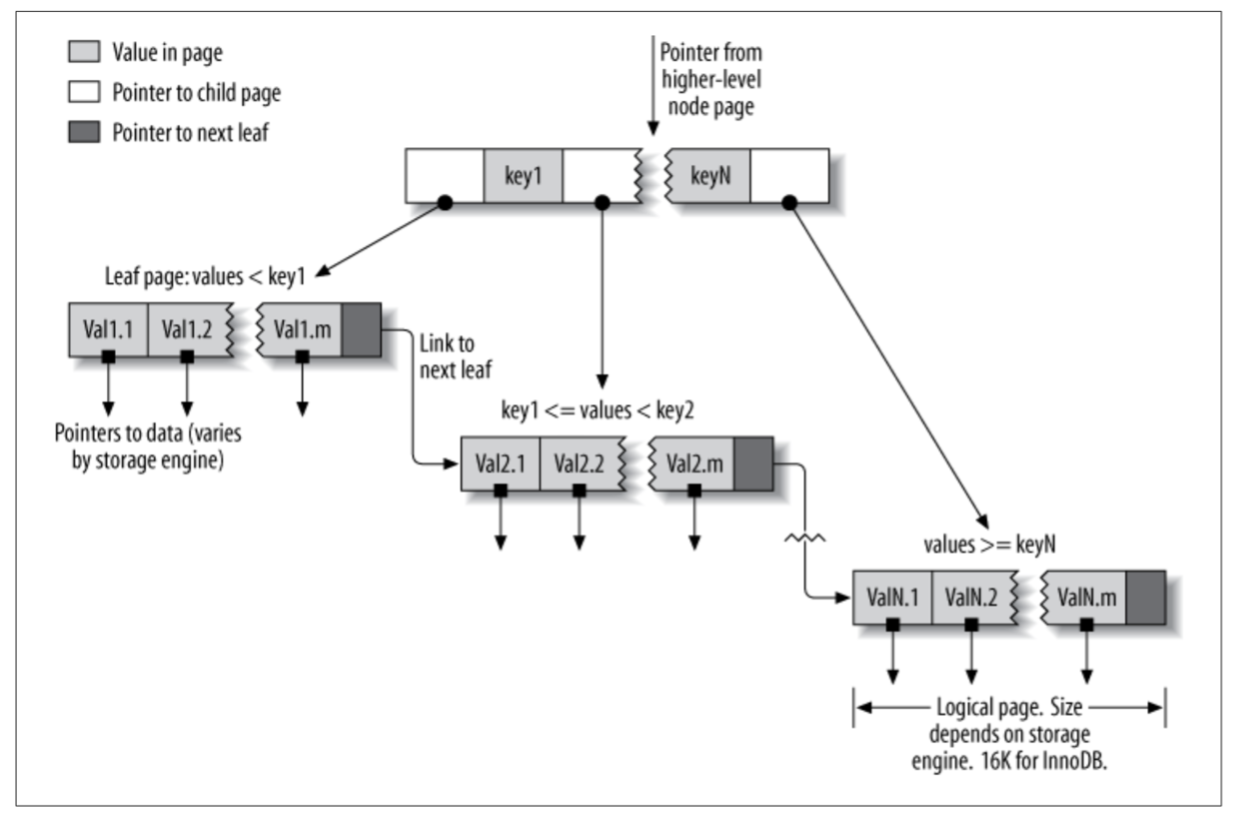
\includegraphics[width=.8\textwidth]{PNGs/B-Tree}
    \caption[Binärbaum - Grafik]{Darstellung des binären Baums mit Knoten und Blättern}
    \label{fig-bad}
\end{figure}

Blattseiten sind besonders, da sie Zeiger auf die indexierten Daten enthalten, anstatt auf andere Seiten zu verweisen.
Zwischen dem Wurzelknoten und den Blattseiten können viele Ebenen von Knoten-Seiten existieren.
Die Tiefe des Baumes hängt von der Größe der Tabelle ab.

Außerdem speichern B-Bäume die indexierten Spalten in einer festgelegten Reihenfolge, was sie besonders nützlich für die Suche nach Datenbereichen macht.
Beispielsweise kann ein Index auf einem Textfeld (z.B. vom Typ \texttt{VARCHAR}) effizient alle Namen finden, die mit „K“ beginnen, da die Werte in alphabetischer Reihenfolge gespeichert sind.

Der Index sortiert die Werte entsprechend der Reihenfolge der in der \texttt{CREATE TABLE}-Anweisung angegebenen Spalten, beispielsweise des Primärschlüssels (\texttt{last\_name, first\_name, b\_day}).
B-Baum-Indizes eignen sich gut für Suchen mit dem vollständigen Schlüsselwert (engl. full key value), einem Schlüsselbereich (engl. key range) oder einem Schlüsselpräfix (engl. full key prefix).
Beim Schlüsselpräfix ist dies jedoch nur der Fall, wenn die Suche das linkeste Präfix des Indexes verwendet.

Als nächstes betrachten wir die möglichen Abfragen, bei denen B-Baum-Indizes besonders hilfreich sind, um ein besseres Verständnis für ihre optimale Nutzung zu erlangen.
Eine Übereinstimmung mit dem vollständigen Schlüsselwert liefert Werte für alle Spalten im Index.
Eine beispielhafte Abfrage wäre die Suche nach allen Einträgen für Max Mustermann, geboren am 2000-01-01, wenn der Schlüssel aus Nachname, Vorname und Geburtsdatum besteht.
Für diesen Index sind auch Abfragen nützlich, die nur mit dem linken Präfix übereinstimmen, beispielsweise die Suche nach „Mustermann“.
Eine weitere Möglichkeit ist die Übereinstimmung mit einem Spaltenpräfix, also dem ersten Teil eines Spaltenwerts, etwa alle Nachnamen, die mit „M“ beginnen.
Ebenso effizient ist der Index bei der Übereinstimmung mit einem Wertebereich, z.B. Nachnamen zwischen „Mustermann“ und „Müller“.

Ein B-Baum-Index kann auch genutzt werden, um Abfragen effizient zu unterstützen, bei denen eine Spalte exakt und eine andere innerhalb eines Wertebereichs abgefragt wird.
Beispielsweise könnte dies eine exakte Übereinstimmung mit dem Nachnamen „Mustermann“ und eine Bereichsabfrage für Vornamen, die mit „Ma“ beginnen, umfassen.
Der letzte Anwendungsfall sind Abfragen, die nur den Index verwenden und nicht die gespeicherten Zeilen, etwa wenn alle benötigten Daten im Index enthalten sind.

Ein weiterer Vorteil von B-Baum-Indizes ist, dass sie aufgrund der sortierten Baumstruktur nicht nur Abfragen, sondern auch \texttt{ORDER BY}-Bedingungen effizient unterstützen können.
Wenn ein B-Baum für die Suche genutzt werden kann, kann er auch für die Sortierung der Ergebnisse verwendet werden.

Es gibt jedoch Einschränkungen von B-Baum-Indizes, die dazu führen, dass andere Indextypen für bestimmte Szenarien besser geeignet sind.
Eine Einschränkung ist, dass die Suche nicht am linken Ende des Indexes beginnen kann.
Beispielsweise ist ein Index, der aus Nachname, Vorname und Geburtsdatum besteht, nicht geeignet, um alle Personen zu finden, die vor dem Jahr 2000 geboren wurden, ohne dass der Nachname und Vorname ebenfalls spezifiziert werden.

Für optimale Leistung sollten Indizes mit den gleichen Spalten, jedoch in unterschiedlicher Reihenfolge erstellt werden, um die häufigsten Abfragen zu optimieren.
Eine Analyse der am häufigsten verwendeten Abfragen kann dabei helfen zu entscheiden, ob zusätzliche Indizes erforderlich sind.
